\documentclass[12pt, letterpaper]{article}

\usepackage[margin=1in]{geometry}
\usepackage{setspace}
\usepackage{parskip}
\usepackage{graphicx}
\usepackage{caption}
\usepackage{hyperref}
\usepackage{natbib}
\usepackage{booktabs}
\usepackage{enumitem}
\usepackage{float}
\usepackage{url}

\onehalfspacing

\title{
    \vspace{2cm}
    \Large\textbf{Probing Secondary Structure and Intrinsic Disorder in Pretrained Protein Language Model Embeddings}\\
    \vspace{0.5cm}
    \large Final Project Report\\
}
\author{Darsh Mandera\\
        \small COMPSCI 590: Computational Biology Seminar\\
        \small Professor Bruce Donald \\
        \small 23 April 2026}
\date{}

\begin{document}

\maketitle
\thispagestyle{empty}
\newpage

\tableofcontents
\newpage

\begin{abstract}
Protein Language Models are transformer-based models pretrained on amino acid sequences that learn biophysical representations without explicit supervision. While they may implicitly encode some biophysical properties, it is unclear which biochemical properties are linearly encoded in PLM embeddings. In this work, we probe ESM-2 embeddings for two properties: secondary structure (a 3-class category consisting of helix, strand, and coil) and intrinsic disorder (a binary category), using linear probes trained on residue-level embeddings. Ultimately, we find that linear probes on ESM-2 embeddings substantially outperform one-hot sequence composition baselines for both properties.
\end{abstract}

\section{Introduction}
Just as natural language processing models treat words (and subword morphemes) as tokens represented by numerical embeddings for predicting and generating text, protein language models (PLMs) treat amino acids as tokens, effectively modeling amino acid sequences as a form of language \citet{chandra2023}. Evolutionary Scale Modeling 2 (ESM-2) is a PLM pretrained on approximately 250 million protein sequences using masked language modeling, where the objective is to predict masked residues from their surrounding context \citet{lin2023esm2}. The ESM-2 architecture is a transformer encoder comprising 12 layers, 35 million parameters, and 480-dimensional residue-level embeddings, with each residue assigned a contextual representation influenced by the entire sequence.
Protein embeddings are analogous to word embeddings in that similar embeddings are expected to reflect similar biophysical contexts (i.e., a form of semantic similarity). However, the extent to which these embeddings capture specific, measurable protein properties remains an open question. In this study, we investigate how well ESM-2 embeddings encode secondary structure and intrinsic disorder.
Secondary structure refers to the local three-dimensional arrangement of the polypeptide backbone. It is typically categorized into three classes—alpha helix (H), beta strand (E), and random coil (C)—which arise from local sequence patterns and hydrogen bonding interactions \citet{pauling1951}. In contrast, intrinsic disorder describes regions of proteins that lack a stable three-dimensional structure under physiological conditions and is often governed by more nonlocal sequence features than secondary structure \citet{habchi2014}.
Here, we assess the extent to which these two properties can be linearly recovered from frozen ESM-2 residue-level embeddings. We use linear probes trained with minimal supervision and compare their performance against a baseline based on one-hot sequence composition.



\section{Methodology}

\subsection{Dataset}
A dataset is loaded via HuggingFace from \texttt{proteinea/secondary\_structure\_prediction} \citet{proteinea_ssp}. This dataset contains 10,792 protein sequences with per-residue annotations across five columns: the amino acid sequence (input), three-class secondary structure labels (\texttt{dssp3: H, E, C}), eight-class secondary structure labels (\texttt{dssp8}), per-residue disorder scores (disorder), and a masking column (\texttt{cb513\_mask}). The disorder column stores space-separated float values (0.0 or 1.0, with some positions marked as ambiguous), and the \texttt{cb513\_mask} column identifies valid sequence positions, as the raw disorder and mask strings are longer than the sequence itself due to formatting. In this work, \texttt{dssp3} is used for secondary structure and disorder is used for intrinsic disorder; input is used as an index for each sequence; \texttt{cb513\_mask} is used as well for preprocessing.

\subsection{Data preprocessing}
A few data preprocessing steps are carried out once the dataset is loaded. First, \texttt{cb513\_mask} is used to align the disorder string to the valid sequence positions. Residues with ambiguous disorder values are discarded. Proteins with fewer than 20 residues are filtered out. Finally, 3,000 proteins are selected for the final dataset.

\subsection{Model and embedding extraction}
The model ESM-2 is loaded from HuggingFace, specifically \texttt{facebook/esm2\_t12\_35M\_UR50D}. It is loaded as a frozen encoder with no fine-tuning, and BOS and EOS tokens are stripped. 480-dimensional embeddings are then extracted from the final layer for each residue across the 3,000 proteins in the working dataset.

\subsection{Linear probe training: ESM-2}
An 80-20 train-test split is performed on the working dataset, yielding 2400 samples for training and 600 for testing. This is then flattened at the residue level. 

A single linear layer is trained with Adam (\texttt{lr=1e-3}), cross-entropy loss, full-batch gradient descent, and 50 epochs for ESM-2 probes. It is worth noting that there is a class imbalance between the two problems, with secondary structure having 3 classes and disorder having 2 classes. Thus, the single linear layer is 480 $\rightarrow$ 3 for secondary structure and 480 $\rightarrow$ 2 for intrinsic disorder. To handle this class imbalance, the disorder probe is trained with inverse-frequency class weighting to prevent majority-class collapse, while the secondary structure probe is trained without weighting. 

\subsection{Baseline}
An identical linear probe architecture is trained on 20-dimensional one-hot amino acid encodings instead of ESM-2 embeddings, with 200 epochs of training used to ensure convergence.

\subsection{Evaluation}
In order to evaluate the models, macro F1 (both per-class and averaged) and AUC (one-vs-rest macro for secondary structure, binary for disorder) are calculated. 

\section{Results}
Overall, we find that both secondary structure and intrinsic disorder are significantly linearly encoded in ESM-2 final-layer embeddings above baseline. The linear probe achieves a similar AUC for both tasks, with a stronger F1 improvement over baseline for secondary structure than for intrinsic disorder.

\begin{table}[h]
\centering
\begin{tabular}{lcccc}
\toprule
 & \multicolumn{2}{c}{Secondary Structure} & \multicolumn{2}{c}{Disorder} \\
\cmidrule(lr){2-3} \cmidrule(lr){4-5}
 & Baseline & ESM-2 Probe & Baseline & ESM-2 Probe \\
\midrule
Macro F1 & 0.359 & 0.707 & 0.428 & 0.637 \\
AUC      & 0.611 & 0.878 & 0.623 & 0.879 \\
\bottomrule
\end{tabular}
\caption{Macro F1 and AUC for ESM-2 probe vs baseline on secondary structure and disorder.}
\label{tab:summary}
\end{table}

\begin{table}[h]
\centering
\begin{tabular}{lcc}
\toprule
Class & Baseline & ESM-2 Probe \\
\midrule
H (helix)  & 0.534 & 0.766 \\
E (strand) & 0.000 & 0.613 \\
C (coil)   & 0.542 & 0.743 \\
\midrule
Macro avg  & 0.359 & 0.707 \\
\bottomrule
\end{tabular}
\caption{Per-class F1 for secondary structure, ESM-2 probe vs baseline.}
\label{tab:ss_perclass}
\end{table}

\begin{table}[h]
\centering
\begin{tabular}{lcc}
\toprule
Class & Baseline & ESM-2 Probe \\
\midrule
Ordered    & 0.139 & 0.362 \\
Disordered & 0.717 & 0.913 \\
\midrule
Macro avg  & 0.428 & 0.637 \\
\bottomrule
\end{tabular}
\caption{Per-class F1 for intrinsic disorder, ESM-2 probe vs baseline.}
\label{tab:dis_perclass}
\end{table}

\subsection{Secondary Structure: ESM-2 probe}

For the secondary structure probe on ESM-2, we find that macro F1 = 0.707 and AUC = 0.878. Per-class F1 results are as follows: helix F1 = 0.766, coil F1 = 0.743, strand F1 = 0.613. Helix and coil are well predicted, with strand being the hardest class having $49\%$ recall. Roughly half of true strands are misclassified, predominantly as coil.

\begin{figure}[H]
    \centering
    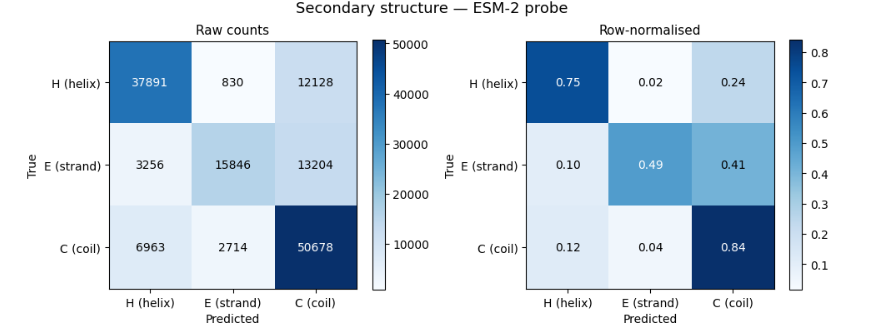
\includegraphics[width=0.8\textwidth]{secondary_structure_confusion_matrix.png}
    \caption{Confusion matrices for the ESM-2 secondary structure probe on the test set. Left: raw counts. Right: row-normalised (recall per class). Rows represent true labels and columns represent predicted labels.}
\end{figure}

\subsection{Secondary Structure: Baseline}
For the secondary structure probe on the baseline, we find that macro F1 = 0.359 and AUC=0.611. The baseline assigns F1=0 to strand entirely, showing that one-hot sequence composition carries no discriminative signal for beta-strands whatsoever.

\subsection{Secondary Structure: Comparison}
Overall, ESM-2 improves macro F1 by +0.349 and AUC by +0.267 over baseline.

\subsection{Disorder: ESM-2 probe}
For the disorder probe on ESM-2, we find that macro F1 = 0.637 and AUC = 0.879. Per-class: disordered F1 = 0.913, ordered F1 = 0.362. The model predicts the majority disordered class well but struggles with ordered residues, reflecting genuine class imbalance.

\begin{figure}[H]
    \centering
    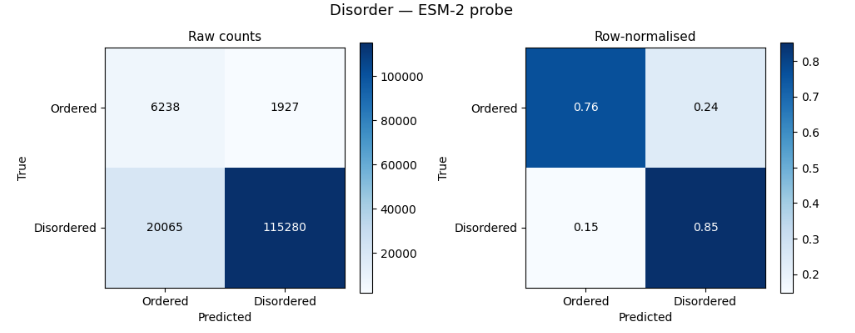
\includegraphics[width=0.8\textwidth]{disorder_confusion_matrix.png}
    \caption{Confusion matrices for the ESM-2 disorder probe on the test set. Left: raw counts. Right: row-normalised (recall per class). Rows represent true labels and columns represent predicted labels.}
\end{figure}

\subsection{Disorder: Baseline}
For the disorder probe on the baseline, we find that macro F1 = 0.428 and AUC = 0.623. 

\subsection{Disorder: Comparison}
Overall, ESM-2 embeddings improve macro F1 by +0.209 and AUC by +0.256 over baseline. The improvement is real but smaller than for secondary structure, and partially confounded by imperfect baseline convergence under class-weighted loss.

\subsection{Protein accuracy vs Protein length}
We find that secondary structure accuracy is flat across all protein lengths, indicating consistent encoding regardless of sequence length. Disorder accuracy increases sharply for proteins up to \textasciitilde{}200 residues then plateaus, suggesting that shorter proteins are harder to classify, possibly due to less contextual signal or a higher proportion of fully disordered short proteins in the dataset.

\begin{figure}[H]
    \centering
    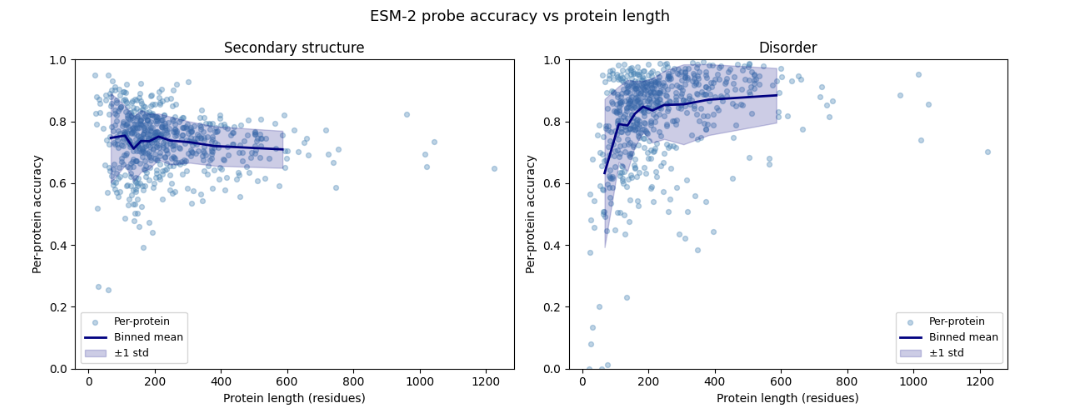
\includegraphics[width=0.8\textwidth]{protein_length_vs_accuracy.png}
    \caption{ESM-2 probe accuracy vs protein length for secondary structure (left) and intrinsic disorder (right). Each point represents one test protein; the navy line shows the binned mean and the shaded region shows ±1 standard deviation.}
\end{figure}



\section{Discussion}
Overall, ESM-2 embeddings appear to linearly encode both secondary structure and disorder over a baseline. This confirms that pretraining on evolutionary sequence data implicitly captures biophysical semantics, despite a lack of explicit pretraining on a biophysical model. When looking at the F1 scores alone, it appears that secondary structure has a greater improvement than disorder. However, this could be credited to the class imbalance in the disorder task. Comparing AUC for both tasks suggests that the final layer of ESM-2 encodes both secondary structure and intrinsic disorder with similar strength. Strikingly, beta-strand identity, completely unrecoverable from sequence composition alone (baseline F1 = 0.000), is clearly linearly encoded in ESM-2 embeddings (F1 = 0.613), demonstrating that transformer-based pretraining on evolutionary sequences captures structural information that cannot be reduced to amino acid composition.

\subsection{Limitations}
One limitation of this work is that only the final layer of ESM-2 is examined. A layerwise probing and analysis could potentially reveal further insights, for example, at which layer each property emerges. Further, to create a memory-effective analysis, only 3,000 proteins are used out of the 10,792 available in the original dataset; an extension of this work could use a larger portion of the dataset. 

\subsection{Future Work}
Future work could address the two key limitations above by performing layerwise probing on a larger portion of the dataset. Additionally, it could be interesting to scale to larger ESM-2-family models; this study uses ESM-2 35M, but larger models may yield different results. Further, this work could be extended to more biophysical properties, such as thermostability which would capture a more global view of proteins.

\section{Project files}
All code, data, and analysis files relevant to this project can be found at \url{https://github.com/dsmandera/cs590-comp-bio-protein-language-model-project}.

\newpage
\bibliographystyle{plainnat}
\bibliography{references}

\end{document}